% ============================================================
%  Section 4.2 – Statistiques descriptives (variables qualitatives)
%  Formules : Chapitre 1 du cours SM403
% ============================================================

\subsection{Statistiques descriptives -- variables qualitatives}

Les trois variables qualitatives retenues sont de type ordinal (Déf.~1.3) :
\textbf{V6 -- Heures de sommeil}, \textbf{V12 -- Moyenne au bac} et
\textbf{V14 -- Assiduité aux CMs}.
Pour chacune, on donne le tableau de fréquences (\(f_i = n_i/n\), Déf.~1.8)
et le mode \(M_o\) (Déf.~1.7).

% ── V6 ──────────────────────────────────────────────────────────────────────
\paragraph{V6 -- Heures de sommeil avant un DE (\(n = 68\)).}

\(M_o = \text{``4--6 h''}\) (\(n_i = 24\), \(35{,}3\,\%\)).
En regroupant les trois premières modalités, \(80{,}9\,\%\) des répondants
dorment moins de 7~heures avant un DE.

\begin{table}[H]
  \centering
  \caption{Fréquences et distribution de V6 -- Sommeil (\(n = 68\))}
  \label{tab:v6}
  \begin{minipage}[t]{0.38\linewidth}
    \vspace{0pt}
    \small\centering
    \begin{tabular}{@{}lrr@{}}
      \toprule
      Modalité     & \(n_i\) & \(f_i\) (\%) \\
      \midrule
      Moins de 4 h & 10 & 14{,}7 \\
      4--6 h       & 24 & 35{,}3 \\
      6--7 h       & 21 & 30{,}9 \\
      7--8 h       &  8 & 11{,}8 \\
      Plus de 8 h  &  5 &  7{,}4 \\
      \bottomrule
    \end{tabular}
  \end{minipage}
  \hfill
  \begin{minipage}[t]{0.40\linewidth}
    \vspace{0pt}
    \centering
    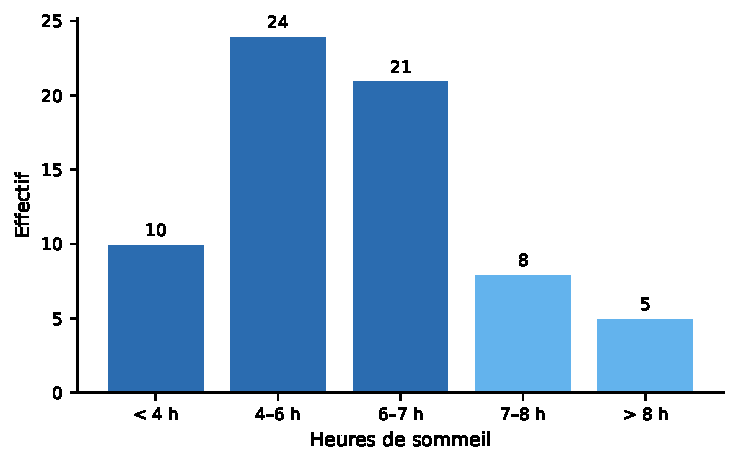
\includegraphics[width=\linewidth]{figures/bar_v6.pdf}
  \end{minipage}
\end{table}

% ── V12 ─────────────────────────────────────────────────────────────────────
\paragraph{V12 -- Moyenne au bac en spécialités scientifiques (\(n = 67\)).}

\(M_o = \text{``12--14''}\) (\(n_i = 39\), \(58{,}2\,\%\)) : distribution très concentrée sur la modalité centrale.

\begin{table}[H]
  \centering
  \caption{Fréquences et distribution de V12 -- Note bac (\(n = 67\))}
  \label{tab:v12}
  \begin{minipage}[t]{0.38\linewidth}
    \vspace{0pt}
    \small\centering
    \begin{tabular}{@{}lrr@{}}
      \toprule
      Modalité & \(n_i\) & \(f_i\) (\%) \\
      \midrule
      8--11    & 13 & 19{,}4 \\
      12--14   & 39 & 58{,}2 \\
      15--17   & 12 & 17{,}9 \\
      18--20   &  3 &  4{,}5 \\
      \bottomrule
    \end{tabular}
  \end{minipage}
  \hfill
  \begin{minipage}[t]{0.40\linewidth}
    \vspace{0pt}
    \centering
    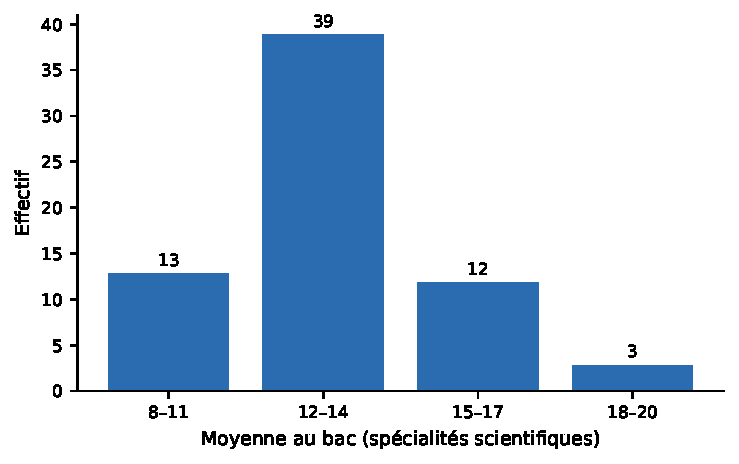
\includegraphics[width=\linewidth]{figures/bar_v12.pdf}
  \end{minipage}
\end{table}

% ── V14 ─────────────────────────────────────────────────────────────────────
\paragraph{V14 -- Assiduité aux cours magistraux (\(n = 68\)).}

\(M_o = \text{``Presque tous''}\) (\(n_i = 33\), \(48{,}5\,\%\)) ;
\(\hat{p}(\text{Tous}) = 29/68 \approx 42{,}6\,\%\).

\begin{table}[H]
  \centering
  \caption{Fréquences et distribution de V14 -- Assiduité aux CMs (\(n = 68\))}
  \label{tab:v14}
  \begin{minipage}[t]{0.38\linewidth}
    \vspace{0pt}
    \small\centering
    \begin{tabular}{@{}lrr@{}}
      \toprule
      Modalité     & \(n_i\) & \(f_i\) (\%) \\
      \midrule
      Rarement     &  6 &  8{,}8 \\
      Presque tous & 33 & 48{,}5 \\
      Tous les CMs & 29 & 42{,}6 \\
      \bottomrule
    \end{tabular}
  \end{minipage}
  \hfill
  \begin{minipage}[t]{0.40\linewidth}
    \vspace{0pt}
    \centering
    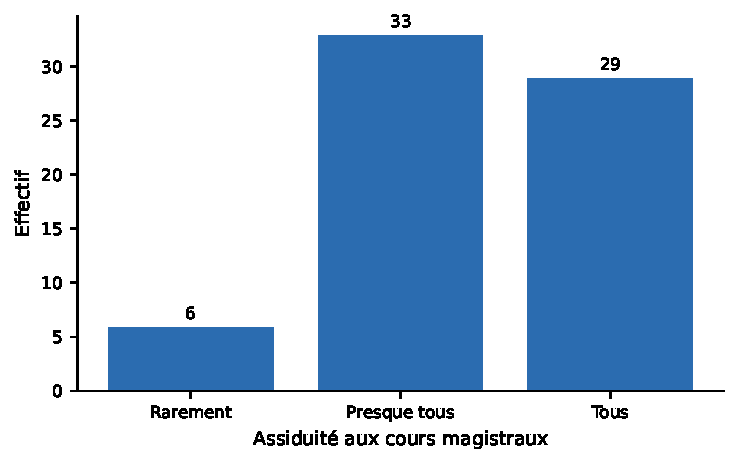
\includegraphics[width=\linewidth]{figures/bar_v14.pdf}
  \end{minipage}
\end{table}
